
\subsection{Ejercicios}
\begin{itemize}
 \item \textbf{Ejercicio 1 } Programar un tipo de tarea TaskConsola, que simular\'{a} una tarea interactiva.
La tarea debe realizar n llamadas bloqueantes, cada una de una duraci\'{o}n al azar 1 entre bmin
y bmax (inclusive). La tarea debe recibir tres par\'{a}metros: n, bmin y bmax (en ese orden)
que ser\'{a}n interpretados como los tres elementos del vector de enteros que recibe la funci\'{o}n.
Explique la implementaci\'{o}n realizada y grafique un lote que utilice el nuevo tipo de tarea.
\item \textbf{Ejercicio 2} El grupo de competencia de Data Mining, reciente ganador de importante concurso internacional, esta
preparando el algoritmo para su próxima victoria. Para esto necesita utilizar fuertemente la CPU por 500 ciclos.
A su vez, el grupo usa la máquina como servidor remoto, utilizando 3 usuarios que realizan llamadas bloqueantes de 10, 20 y 30 
respectivamente y de una duración al azar de hasta 4 ciclos.
Escribir el lote de tareas que simule la situación del grupo. Ejecutar y graficar la simulación usando el algoritmo FCFS para 1 y 2 y 4 
núcleos con un cambio de contexto de 5 ciclos. Calcular la latencia de cada tarea en los dos gráficos. Explicar 
que desventaja tendría si debe mantener este algoritmo de scheduling y solo tiene disponible una computadora con un núcleo (haga
referencia a los gráficos y a los cálculos anteriores para justificar su explicación).

\item \textbf{Ejercicio 3} Programar un tipo de tarea TaskBatch que reciba dos par\'{a}metros: total cpu y
cant bloqueos. Una tarea de este tipo debera realizar cant bloqueos llamadas bloqueantes, en
momentos elegidos pseudoaleatoriamente. En cada tal ocasi\'{o}n, la tarea deber\'{a} permanecer
bloqueada durante exactamente dos (4) ciclos de reloj. \\
El tiempo de CPU total que utilice una
tarea TaskBatch deber\'{a} ser de total cpu ciclos de reloj (incluyendo el tiempo utilizado para
lanzar las llamadas bloqueantes; no as\'{i} el tiempo en que la tarea permanezca bloqueada).
Explique la implementaci\'{o}n realizada y grafique un lote que utilice 4 tareas TaskBatch con
par\'{a}metros diferentes y que corra con el scheduler FCFS.
\end{itemize}

\subsection{Resultados y Conclusiones}

\subsubsection[Resolución Ejercicio 1]{Ejercicio 1}

\indent Dada la simpleza del código, optamos por mostrar nuestra implementación, en vez de comentarlo\\ detalladamente.\\
\indent Realizamos un ciclo de i \textless \ params[0], donde utilizamos la función dada por la catedra, uso\_IO a la cual le pasamos
el pid correspondiente y un entero ciclos que es el valor random obtenido entre $bmin$ y $bmax$. Esa función uso\_IO simula una llamada bloqueante.
\begin{center}
 \begin{verbatim}
                     ciclos = rand() % (params[2] - params[1] + 1) + params[1];
 \end{verbatim}

\end{center}

\indent A continuaci\'{o}n, el c\'{o}digo mencionado:

\begin{verbatim}

                  void TaskConsola(int pid, vector<int> params) {
                       int i, ciclos;              
                       for (i = 0; i < params[0]; i++) {
                              ciclos = rand() % (params[2] - params[1] + 1) + params[1];  
                              uso_IO(pid, ciclos);
                       }
                  } 

\end{verbatim}

\indent Como experimentaci\'{o}n trabajamos con el siguiente lote:\\

\begin{verbatim}
                              TaskConsola 5 3 7
                              TaskConsola 2 3 3
                              TaskConsola 15 2 7
\end{verbatim}

De aqu\'{i}, obtuvimos los siguientes resultados:\\

\vspace*{0.3cm} \vspace*{0.3cm}
  \begin{center}
 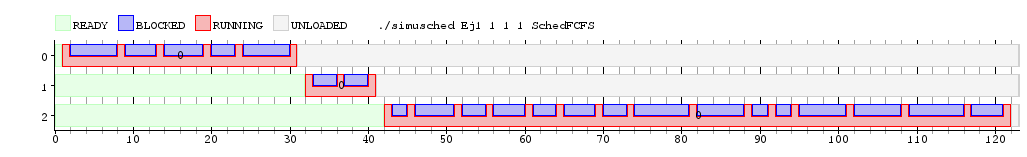
\includegraphics[scale=0.5]{./Test/ej1.png}
 { $Gr$\'a$fico 1.1$ Scheduler FCFS - 1 core }
 \end{center}
  \vspace*{0.3cm}



\subsubsection[Resolución Ejercicio 2]{Ejercicio 2}


\indent ESTE HAY QUE HACERLO

\subsubsection[Resolución Ejercicio 3]{Ejercicio 3}

EN ESTE EJERCICIO HAY Q CAMBIAR EL USO IO DE 1 A 4 Y CAMBIAR EL EXPERIMENTO

\indent Al igual que con la tarea TaskConsola, mencionaremos nuestro implementación y por consiguiente  
explicaremos ciertos puntos de la misma.\\
 \begin{verbatim}
                       void TaskBatch(int pid, vector<int> params) {
                            int total_cpu = params[0];
                            int cant_bloqueos = params[1];
                            vector<bool> uso = vector<bool>(total_cpu);
                            for(int i=0;i<(int)uso.size();i++) 
                               uso[i] = false;
                               for(int i=0;i<cant_bloqueos;i++) {
                                  int j = rand()%(uso.size());
                                  if(!uso[j])
                                     uso[j] = true;
                                  else
                                     i--; 
                               }
                               for(int i=0;i<(int)uso.size();i++) {
                                  if( uso[i] )
                                     uso_IO(pid,1); 
                                  else
                                     uso_CPU(pid, 1); 
                               }
                       }
 \end{verbatim}

 \indent Para este tipo de tarea, creamos un vector de tamaño igual a $total\_cpu$ el cual contiene valores booleanos, 
 si el valor en el \'{\i}ndice del vector es true este corresponder\'a a la funci\'{o}n uso\_IO, caso contrario uso\_CPU.\\
 Luego, utilizaremos un ciclo que irá desde 0 hasta el tamaño del vector y dependiendo el valor booleano, usará la funciones
 dadas por la catedra uso\_IO o uso\_CPU.\\
 
 \indent El experimento realizado para este nuevo tipo de tarea fue el siguiente:\\
 
 Con un lote de tareas:\\
 
 \begin{verbatim}
                           TaskBatch 10 3
                           TaskBatch 5 4
                           TaskBatch 8 1
 \end{verbatim}

 Obtuvimos el siguiente diagrama:\\
 
 \vspace*{0.3cm} \vspace*{0.3cm}
  \begin{center}
 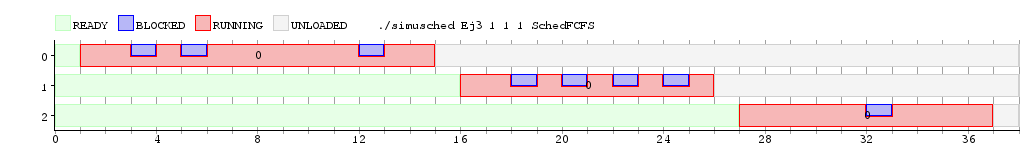
\includegraphics[scale=0.5]{./Test/ej3.png}
 { $Gr$\'a$fico 3.1$ Scheduler FCFS - 1 core }
 \end{center}
  \vspace*{0.3cm}
 
